%%% LaTeX Template: Article/Thesis/etc. with colored headings and special fonts
%%%
%%% Source: http://www.howtotex.com/

\documentclass[12pt]{article}


\usepackage{apuntes-estilo}
\usepackage{fancyhdr,lastpage}



\def\maketitle{

% Titulo 
 \makeatletter
 {\color{bl} \centering \huge \sc \textbf{
 Aprendiendo Vim Progresivamente \\ 
 \vspace*{8pt} }\par}
 \makeatother


% Autor
 \makeatletter
 {\centering \small 
 	Departamento de Ingeniería de Computadoras \\
 	Facultad de Informática - Universidad Nacional del Comahue \\
 	\vspace{20pt} }
 \makeatother

}

% Custom headers and footers
\fancyhf{} % clear all header and footer fields
\fancypagestyle{plain}{\fancyhf{}}
  	\pagestyle{fancy}
 	\lhead{\footnotesize Aprendiendo Vim Progresivamente - Departamento de Ingeniería de Computadoras}
 	\rhead{\footnotesize \thepage\ }	% ``Page 1 of 2''

\def\ti#1#2{\texttt{#1} & #2 \\ }



\begin{document}

\thispagestyle{empty}
\maketitle
\setlength{\parindent}{0pt}


Este tutorial fue pensado como una guía mínima, para aprender a utilizar el editor Vim 
\footnote{http://www.vim.org}
en el menor tiempo posible. La idea es la siguiente : primero, se debe aprender lo mínimo para sobrevivir,
y luego, de a poco, aprender nuevos comandos útiles.

Aprender Vim es difícil, pero increíblemente eficiente cuando se lo utiliza.

\section{Introducción}

Vim es un editor de texto de gran utilidad para los administradores de sistemas ya
que está disponible en cualquier plataforma UNIX. Esto significa
que podrá usar Vim en cualquier sistema de tipo UNIX. Además,
resulta recomendable su utilización, porque requiere de muy pocos
recursos para su funcionamiento, lo que permite utilizar Vim
en maquinas remotas o cuando no pueda ejecutar otros programas
debido a problemas con el hardware o el sistema.

\fcolorbox{black}{grey}{
\parbox[t]{1.0\linewidth}{ \vspace*{0.4cm}
{\bf Advertencia}. Aprender Vim es muy
pero muy difícil al principio. Tomará tiempo. Será como intentar aprender
a tocar un instrumento de música. Por lo tanto, no sueñe con ser más
eficiente con Vim, en menos de tres días, que con cualquier otro editor que ya conozca.
Es más, conocer Vim de manera eficiente puede tomar dos o más semanas en vez
de sólo tres días.
\vspace*{0.4cm} } }

El tutorial está estructurado en una serie de pasos, como una guía
secuencial para el aprendizaje de Vim. Los cuatro pasos que debe seguir son :

\begin{enumerate}
	\item Sobrevivir
	\item Sentirse cómodo
	\item Sentirse mejor, con confianza, y mas rápido
	\item Utilizar los súper poderes de Vim
\end{enumerate}

\textit{Y cuando esté finalizando este camino será un ¡Vim superstar!.}


\section{Nivel 1 - Sobrevivir}


Pasos:

\begin{enumerate}
	\item Instalar Vim
	\item Ejecutar Vim
	\item ¡NO HAGA NADA!. Sólo lea.
\end{enumerate}

Luego de instalar el editor Vim inicie su ejecución. Puede hacerlo
escribiendo vim[ENTER] en una terminal.

Aquí está la primer lección difícil de entender si es su primer contacto
con Vim : cualquier intento de mover el cursor o de escribir, como lo haría con cualquier otro
editor, no funcionará.

Si intenta moverse por la
pantalla comprobaremos además, que las teclas del cursor no hacen nada, y que el
ratón tampoco responde. ¿Qué ocurre? 

\textbf{Lo que ocurre es que Vim tiene diferentes modos de funcionamiento.
Y, de manera predeterminada, inicia en \textit{Modo Normal}}.


\subsection{Modos Fundamentales de Vim}

Los dos modos fundamentales son los llamados modos normal y de inserción. 
El \textbf{Modo Normal} es aquel
en el que Vim se encuentra al iniciar y en el que se supone que debemos
dejarlo cuando no estemos haciendo otra cosa (por eso se llama normal). En él
cualquier pulsación de teclas que realicemos se interpretará como comando. Por
el contrario en el \textbf{Modo de Inserción} Vim se comporta como cualquier
otro editor de texto, es decir: las teclas que presionamos se irán mostrando en
pantalla en el lugar donde estaba el cursor, siendo interpretado como texto que
hay que introducir en el documento que estamos editando.

Debemos hacer notar que Vim llama modo normal a aquel en el que menos se
parece a otros editores de texto. Tal vez por ello a veces a este modo se le
llama también \textit{Modo de Comando}, aunque el nombre de modo normal es bastante
indicativo de la filosofía de Vim. La idea es que siempre que no estemos
haciendo otra cosa activemos el modo normal: mientras revisamos el texto
escrito, mientras reflexionamos sobre qué añadir, mientras contestamos al
teléfono, si hacemos una pausa para tomar un mate...
se supone que habremos activado el modo normal.

Para ingresar al Modo Inserción, el cual es muy parecido al funcionamiento
de cualquier otro editor, simplemente debe presionar la letra ``i''.
Ahora debería sentirse un poco mejor, ya que en Modo Inserción puede
escribir de manera similar a un editor típico.

Para salir del Modo Inserción, y volver al Modo Normal sólo necesita
presionar la tecla ESC.

\fcolorbox{black}{grey}{
\parbox[t]{1.0\linewidth}{ \vspace*{0.4cm}
{\bf Recuerde: con las teclas i y ESC, puede cambiar entre el Modo
Normal y el Modo Inserción.}
Detectará que está en modo Inserción
porque sobre la esquina inferior izquierda de la ventana de Vim se leerá
\texttt{INSERT} o \texttt{INSERCION}. Al presionar ESC y volver al Modo Normal
no habrá ninguna leyenda.
\vspace*{0.4cm} } }


\begin{itemize}
	\item Ahora es el momento de que aprenda lo necesario para sobrevivir
en Modo Normal : \\ \\
\begin{tabular}{ l l l }
	\ti{:q[ENTER]}{salir del editor}
	\texttt{i} &  cambia el modo al Modo Inserción. Presione ESC para volver al Modo Normal \\
	\texttt{x} &  borrar el caracter bajo el cursor \\
	\texttt{:wq[ENTER]} & guardar y Salir (:w guardar, :q salir) \\
	\texttt{dd} &  borrar (y copiar) la línea actual \\
	\texttt{p} &  pegar \\
\end{tabular}
\end{itemize}

	

\begin{itemize}
	\item Recomendados : \\ \\
\begin{tabular}{ l l }
	\texttt{h} & mueve el cursor a la izquierda \\
	\texttt{j} & mueve el cursor hacia abajo \\
	\texttt{k} & mueve el cursor hacia arriba \\
	\texttt{l} & mueve el cursor a la derecha \\
\end{tabular}
\end{itemize}

\begin{itemize}
	\item Obteniendo ayuda: \\ \\
\begin{tabular}{ l l }
	\texttt{:help <comando>[ENTER]}  & Muestra la ayuda acerca del \texttt{<comando>}. Puede utilizar \texttt{:help} sin \texttt{<comando>} para obtener ayuda en general. \\
\end{tabular}
\end{itemize}

Sólo necesita aprender estos ocho comandos del Modo Normal para sobrevivir y comenzar.
Luego, cuando se sienta cómodo con estos comandos (tal vez en un día o dos), puede continuar con el nivel 2.


\fcolorbox{black}{grey}{
\parbox[t]{1.0\linewidth}{ \vspace*{0.4cm}
{\bf Familiarizarse con el Modo Normal.} En otros
editores, para copiar texto se debe presionar la tecla Ctrl
(generalmente Ctrl-C). Más aún, cuando presiona Ctrl en esos editores,
es como si todas las teclas cambiaran
de significado. Usando Vim en Modo Normal es similar a lo anterior, como si
automáticamente Vim presionara la tecla Ctrl por usted.
\vspace*{0.4cm} } } 


Una última palabra acerca de las notaciones :

\begin{itemize}
	\item En vez de escribir Ctrl-, escribiremos en este documento \texttt{<C- >}.
	\item Los comandos que comienzan con ``:'' finalizan con \texttt{<ENTER>}. Por ejemplo,
cuando lea :q usted debe escribir :q y presionar \texttt{<ENTER>}
\end{itemize}


\section{Nivel 2 - Sentirse Cómodo}


Si ya se siente cómodo con los comandos necesarios para sobrevivir 
puede continuar y aprender unos pocos comandos más. Estos son los sugeridos:


\begin{itemize}
	\item Variantes para ingresar al Modo Inserción: \\ \\
\begin{tabular}{ l l }
            \texttt{a} & ingresa al modo inserción y se posiciona en la siguiente posición a partir del cursor \\
            \texttt{o} & agregar una nueva línea vacía e ingresa al modo inserción \\
            \texttt{O} & agregar una nueva línea antes de la línea actual, e ingresa al modo inserción \\
            \texttt{cw} & ingresa al modo inserción reemplazando la palabra actual \\
\end{tabular}
\end{itemize}



\begin{itemize}
	\item Movimientos Básicos: \\ \\
\begin{tabular}{ l l }
            \texttt{0} & saltar al primer caracter de la linea \\
            \texttt{\^} & saltar al primer caracter no blanco de la linea \\
            \texttt{\$} & saltar al fin de linea \\
            \texttt{g\_} & saltar al último caracter no blanco de la linea \\
            \texttt{/pattern} & buscar en el documento actual el texto \texttt{pattern} \\
\end{tabular}
\end{itemize}



\begin{itemize}
	\item Copiar y Pegar: \\ \\
\begin{tabular}{ l l }
            \texttt{P} & pegar antes, ya que p es pegar después de la posición del cursor \\
            \texttt{yy} & copiar la línea actual, mas fácil pero equivalente a \texttt{ddP} \\
            \texttt{u} & undo \\
            \texttt{<C-r>} & redo \\
\end{tabular}
\end{itemize}


\begin{itemize}
	\item Cargar/Guardar/Salir/Cambiar Archivo(Buffer): \\ \\
\begin{tabular}{ l l }
            \texttt{:e <path/to/file>} & abrir \\
            \texttt{:w} & guardar \\
            \texttt{:saveas <path/to/file>} & guardar a \texttt{<path/to/file>} \\
            \texttt{:x}, \texttt{ZZ} o \texttt{:wq} & guardar y salir (\texttt{:x} solamente guardar si es necesario) \\
            \texttt{:q!} & salir sin guardar, también: \texttt{:qa!} para salir aun si hubieron buffers ocultos modificados \\
            \texttt{:bn} (o \texttt{:bp}) & mostrar el siguiente archivo (o el anterior) (buffer) \\
\end{tabular}
\end{itemize}



Tome el tiempo que sea necesario para aprender estos comandos,
ya que una vez que los conozca podrá trabajar con Vim como lo
hace con cualquier otro editor. Puede que aún se sienta un poco incómodo 
con la dificultad inicial y la manera en que Vim trabaja, pero verá
que luego del siguiente nivel Vim le devolverá con creces el trabajo
de haberlo aprendido.


\section{Nivel 3 - Mejor. Más Fuerte. Más Rápido.}


¡Felicitaciones por llegar hasta aquí!, ahora empieza la parte interesante.
En el Nivel 3 veremos únicamente comandos compatibles con el viejo editor vi.


\subsection{Mejor}


\begin{itemize}
	\item Vea como Vim lo puede ayudar a realizar tareas repetitivas: \\ \\
\begin{tabular}{ l l }
	\texttt{.} & (punto) repetirá el último comando \\
	\texttt{N<command>} & repetirá el comando \texttt{<command>} N veces \\
\end{tabular}
\end{itemize}


\subsubsection{Ejercitación}


\begin{itemize}
	\item Inicie Vim y escriba : \\ \\
\begin{tabular}{ l l }
	\texttt{2dd} & borrará 2 líneas \\
	\texttt{3p} & pegará el texto 3 veces \\
	\texttt{100idesu [ESC] } & escribirá \\
\end{tabular}
\end{itemize}
“desu desu desu desu desu desu desu desu desu desu desu desu desu desu desu desu desu desu desu desu desu desu desu desu desu desu desu desu desu desu desu desu desu desu desu desu desu desu desu desu desu desu desu desu desu desu desu desu desu desu desu desu desu desu desu desu desu desu desu desu desu desu desu desu desu desu desu desu desu desu desu desu desu desu desu desu desu desu desu desu desu desu desu desu desu desu desu desu desu desu desu desu desu desu desu desu desu desu desu desu “
\begin{itemize}
	\item Repetimos el último comando recién ejecutado: \\ \\
\begin{tabular}{ l l }
	\texttt{.} & repite el último comando, por lo que escribirá nuevamente 100 “desu “ \\
	\texttt{3.} & escribirá 3 “desu” (y no 300, que inteligente ¿no?) \\
\end{tabular}
\end{itemize}



\subsection{Más fuerte}

Conocer como moverse eficientemente con Vim es muy importante. No saltee esta
sección.

\begin{itemize}
	\item Saltos entre líneas:  \\ \\
\begin{tabular}{ l l }
	\texttt{NG} & saltar a la linea N (equivalente a \texttt{:N}\\
	\texttt{gg} & lo mismo que \texttt{1G} o \texttt{:0} - saltar al inicio del archivo \\
	\texttt{G} & saltar a la ultima línea \\
\end{tabular}
\end{itemize}




\begin{itemize}
	\item Movimiento entre palabras: \\ \\
\begin{tabular}{ l l }
	\texttt{w} & ir al inicio de la siguiente palabra \\
	\texttt{e} & saltar al final de la palabra actual \\
	\texttt{b} & saltar al comienzo de la palabra actual \\
\end{tabular}
\end{itemize}



	De manera predeterminada, para Vim, las palabras están compuestas de letras y del caracter ``\_''. 
Digamos que una PALABRA es un grupo de letras separadas por un caracter blanco. 

\begin{itemize}
	\item Si sólo desea trabajar con PALABRAS entonces utilice únicamente caracteres en mayúsculas: \\ \\
\begin{tabular}{ l l }
	\texttt{W} & saltar al inicio de la siguiente PALABRA \\
	\texttt{E} & saltar al final de la PALABRA actual \\
\end{tabular}
\end{itemize}

\begin{center}
 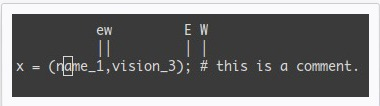
\includegraphics{./img/wordWORD.jpg}
 % redireccionamiento.gif: 502x248 pixel, 72dpi, 17.71x8.75 cm, bb=0 0 502 248
\end{center}

	
\begin{itemize}
	\item Ahora debe aprender a realizar movimientos muy eficientes: \\ \\
\begin{tabular}{ l l }
	\texttt{\%} & saltar a la correspondencia de \texttt{(, \{, [ }  \\
        \texttt{* (o \#)} & ir a la próxima (o previa) ocurrencia de la palabra bajo el cursor \\
\end{tabular}
\end{itemize}


Para recordar : los últimos 3 comandos son oro puro.

\subsection{Más Rápido}

La razón de la importancia de los movimiento en vi tiene una razón :
La mayoría de los comandos puede ser utilizado usando el formato general siguiente :

\texttt{<posición de inicio><command><posición final>}


\begin{itemize}
	\item Por ejemplo : 0y\$ significa \\ \\
\begin{tabular}{ l l }
	\texttt{0} & ir al comienzo de la linea \\
	\texttt{y} & copiar desde aquí \\
	\texttt{\$} & hasta el fin de la linea actual \\
\end{tabular}
\end{itemize}

También puede ejecutar cosas como ``ye'', copiar desde la posición actual hasta el final de la palabra.
Y también puede ejecutar cosas como ``y2/foo'', lo cual copia hasta la segunda ocurrencia de la palabra ``foo''.

Además, lo que es cierto para \texttt{y} (copiar -en inglés yank-), es también cierto para \texttt{d} (borrar -en inglés delete-), gU (mayúsculas), gu (minúsuclas), etc.

\section{Nivel 4 - Súper poderes de Vim}

Si utiliza todos los comandos anteriores trabajará cómodamente con Vim.
Y además, ahora tiene la preparación necesaria para aprender las características ``matadoras''.  Algunos de los siguientes comandos son la razón por la cual comencé a utilizar Vim.



\begin{itemize}
	\item Movimientos en la linea actual:  0 \^ \$ g\_ f F t T , ; \\ \\
\begin{tabular}{ l l }
	\texttt{0} & saltar a la columna 0 \\
	\texttt{\^} & ir al primer caracter en la linea \\
	\texttt{\$} & saltar al fin de la linea \\
	\texttt{g\_} & saltar al ultimo caracter en la linea \\
	\texttt{fa} & saltar a la próxima ocurrencia de la letra a en la linea. ``,''  (o ``;'') encontrará la próxima ocurrencia o la previa \\

	\texttt{t,} & saltar al caracter anterior a ``,'' \\
	\texttt{3fa} & encontrar la 3er ocurrencia de una a en la linea \\
	\texttt{F y T} & actúan de la misma manera que ``f''  y ``t'' pero en reversa \\
\end{tabular}
\end{itemize}

\begin{center}
 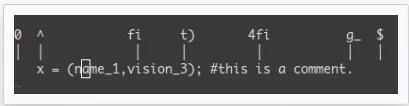
\includegraphics{./img/movecurrline.jpg}
 % redireccionamiento.gif: 502x248 pixel, 72dpi, 17.71x8.75 cm, bb=0 0 502 248
\end{center}



Un tip útil es: \texttt{dt"}  el cual borra todo hasta el caracter ".

\subsection{Selección de una Zona \texttt{<action>a<object> o <action>i<object>}}


Estos comandos pueden sólo ser utilizados después de un operador en Modo Visual. Pero son muy poderosos. Su principal patrón es :

\texttt{<action>a<object> y <action>i<object>}


Donde action puede ser cualquier acción, por ejemplo, d (delete), y (copiar), v (seleccionar en modo visual). El objeto (object) puede ser : w para una palabra, W para una PALABRA (palabra extendida), s para una sentencia, p para un párrafo. Y también, caracteres naturales, tales como \texttt{", ', ), \}, ] }.


\begin{itemize}
	\item Suponga que el cursor esta en la primer ``o'' que aparece en  (map (+) (``foo'')) \\ \\
\begin{tabular}{ l l }
	\texttt{vi"} & seleccionará foo. \\
	\texttt{va"} & seleccionará "foo" \\
	\texttt{vi)} & seleccionará ``foo'' \\
	\texttt{va)} & seleccionará (``foo'') \\
	\texttt{v2i)} & seleccionará map (+) (``foo'') \\
	\texttt{v2a)} & seleccionará (map (+) (``foo'')) \\
\end{tabular}
\end{itemize}


\begin{center}
 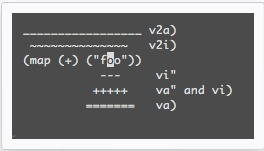
\includegraphics{./img/vivisual.jpg}
 % redireccionamiento.gif: 502x248 pixel, 72dpi, 17.71x8.75 cm, bb=0 0 502 248
\end{center}


\subsection{Selección de bloques rectangulares: \texttt{<C-v>}}

Los bloques rectangulares son muy útiles para comentar muchas
líneas de código. Típicamente:  \texttt{0<C-v><C-d>I-- [ESC]}

\begin{itemize}
	\item Ejemplo: \\ \\
\begin{tabular}{ l l }
	\texttt{\^} & ir al principio de la linea \\
	\texttt{<C-v>} & Comenzar con la selección de un bloque \\
	\texttt{<C-d>} & Mover hacia abajo la selección (también podría ser jjj o \%, etc…) \\
	\texttt{I-- [ESC]} & escribir -- al comentario de cada linea \\
\end{tabular}
\end{itemize}




\subsection{Completar: \texttt{<C-n> y <C-p>}}


En Modo Inserción, sólo escriba el inicio de una palabra,
y entonces presione \texttt{<C-p>}, Vim completará la palabra mágicamente con
una sugerencia encontrada en el documento actual.


\begin{itemize}
	\item Macros: \\ \\ 
\begin{tabular}{ l l }
	\texttt{qa} & hacer algo q, \texttt{@a, @@}
\end{tabular}
\end{itemize}

qa registra sus acciones en el registro a. Entonces @a ejecutará nuevamente
la macro guardada dentro del registro a, como si la hubiese escrito.

Ejemplo: en una linea que contiene sólo números ``1'', escriba lo siguiente:

\begin{itemize}
	\item Ejemplo. En una linea que contiene sólo números ``1'', escriba lo siguiente: \\ \\
\begin{tabular}{ l l }
	\texttt{qaYp<C-a>q} & recuerde que \texttt{<C-a> es Ctrl+a} \\
\end{tabular}
\end{itemize}
\begin{itemize}
	\item El comando anterior realiza lo siguiente: \\ \\
\begin{tabular}{ l l }
            \texttt{qa} & inicia el registro \\
            \texttt{Yp} & duplica la línea \\
            \texttt{<C-a>} & incrementa el número \\
            \texttt{q} & finaliza el registro de acciones \\
\end{tabular}
\end{itemize}
\begin{itemize}
	\item Y podemos finalizar el ejemplo con: \\ \\
\begin{tabular}{ l l }
	\texttt{@a} & escribe 2 bajo el 1 \\
	\texttt{@@} & escribe 3 bajo el 2 \\
\end{tabular}
\end{itemize}

Ahora escriba 100@@ y eso creará una lista incremental de números hasta el 103.



\subsection{Selección Visual: \texttt{v,V,<C-v>}}


Anteriormente se especificó un ejemplo utilizando \texttt{<C-v>}.
Hay también v y V. 


\begin{itemize}
	\item Una vez que se ha realizado una selección, puede: \\ \\
\begin{tabular}{ l l }
	\texttt{J} & unir todas las lineas juntas \\
	\texttt{< (o >)} & realiza una sangría a la izquierda (o a la derecha) \\
	\texttt{=} & auto realizar la sangría \\
\end{tabular}
\end{itemize}





\begin{itemize}
	\item Agregar contenido al final de todas las líneas visualmente seleccionadas: \\ \\
\begin{tabular}{ l l }
	\texttt{<C-v>} & inicia el modo selección \\
\end{tabular}
\end{itemize}
\begin{itemize}
    \item luego ir a la linea deseada (jjj o \texttt{<C-d> o /pattern o \%} etc…). Finalmente: \\ \\
\begin{tabular}{ l l }
	\texttt{\$} & ir al final de la linea \\
	\texttt{A,} & escribir texto, ESC \\
\end{tabular}
\end{itemize}

Todas las líneas seleccionadas contendrán, al final, el texto recién ingresado.


\subsection{Dividir las pantallas :split y vsplit}

Además de aprender los comandos de esta sección se recomienda leer la ayuda con \texttt{:help split}.

\begin{itemize}
	\item Estos son los comandos mas útiles para dividir la pantalla: \\ \\
\begin{tabular}{ l l }
	\texttt{:split} & crea una división (:vsplit crea una división vertical) \\
	\texttt{<C-w><dir>} & donde dir es cualquiera de las teclas de movimiento hjkl o los cursores de movimiento para cambiar la división \\
	\texttt{<C-w>\_ (o <C-w>|)} & maximiza el tamaño de la división (o la división vertical) \\
	\texttt{<C-w>+ (o <C-w>-)} & Expande (o achica) la división \\
\end{tabular}
\end{itemize}



\section{Conclusión}

En este documento se explica el 90\% de los comandos que utilizo a diario. Se sugiere que no aprenda mas de uno o dos comandos por día. Después de dos o tres semanas comenzará a sentir el poder de Vim en sus manos.

Aprender a utilizar Vim es una tarea de entrenamiento, no de memorización. Afortunadamente para ello, Vim 
provee buenas herramientas y excelente documentación. Ejecute vimtutor hasta que esté familiarizado con los comandos básicos. Y también, debería leer esta ayuda cuidadosamente:  \texttt{:help usr\_02.txt}.

Ahí aprenderá acerca de !, directorios, registros, plugins y muchas otras cosas. Estudie Vim como si estuviese aprendiendo a tocar el piano y todo irá bien.

\section{Licencia}
Este documento es una traducción y adaptación del documento
original ``Learn Vim Progressively''
\footnote{http://yannesposito.com/Scratch/en/blog/Learn-Vim-Progressively/}
 - distribuido con licencia
Attribution-ShareAlike 3.0 Unported (CC BY-SA 3.0) - 
http://creativecommons.org/licenses/by-sa/3.0/

\end{document}
